\chapter{Distributed VoIP platform design}
\label{ch:platform}
http://blog.2600hz.com/post/5399315067/erlang-and-freeswitch-the-future-of-cloud

\section{Why Erlang?}
We spent a lot of time looking for all the pieces above. Foolishly, we were looking for them individually. We thought of using beanstalk and Java or even Amazon’s hosted service for messaging. All of them would require setting up our own queues and brokering systems. Some cost money. We thought about using PHP and lighthtppd / nginx / Apache for the web portions. We thought about using the event socket and something (we never did figure that out) for the real-time streaming. We played with Comet extensively for the browser component and tried out XML and JSON.

But all in all, everything felt cobbled together and there were always large gaps.

We didn’t just read about these technologies, either - we’ve actually tried many different languages (Perl, Python, PHP, Ruby) as well as databases (Postgres, MySQL, SQLite, MongoDB, CouchDB). Only through trial and error have we really been able to assess the strengths and weaknesses of each platform through use of specific VoIP applications - not just general research and theory.

When we found Erlang: It literally was like heaven when we began exploring it’s capabilities. It excelled in every single item we listed above out-of-the-box and in the last three years has seen much expansion on it’s few weaknesses. For example, the built-in Mnesia database system was really not acceptable for our purposes and required too much manual labor to maintain, but CouchDB (also written in Erlang) would fill that gap. RabbitMQ filled any gaps in messaging, and FreeSWITCH already had an Erlang connector. 

It was a no brainer to dive into this technology, and it has served us very well in both reliability and scalability.

\section{Platform design}

-OpenSIPs
-FreeSWITCH
-Whistle
-RabbitMQ
-WhApps

wh-msg
ecallmgr

We will soon begin posting statistics and information about our findings with Erlang in great depth, but in the meantime, let’s just say that it’s exceeded all expectations.  

After researching many languages and options, we basically ended up with two choices. Option one was to code our platform in C, making it more popular and easier to tie in with other code libraries but likely to require months of work designing a highly scalable distributed threading and messaging system ourselves (or integrate with one like ZeroMQ) along with threading, supervision and parsing engines. Option two was to use a programming language where someone had already done all that work to help give us a head-start, in the hopes that the language itself would increase in popularity as others began facing similar problems as listed above.

We chose the latter. Since doing so, Erlang’s popularity has grown, and we’re convinced it was the right choice to get us moving in the right direction. 

Here’s what Erlang gave us for free:

*Powerful Messaging
*Powerful Data Storage
*Native types and connections between messaging and data storage engines
*Ability to Swap Code on Running Systems (0 downtime as a goal)
*Ability to Distribute Compiled Code Cross-Platform
*Massively scalable processes/threading

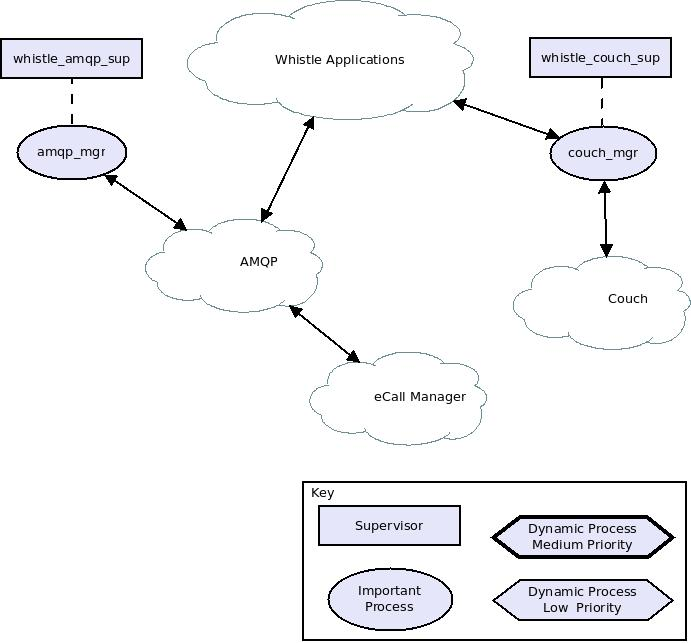
\includegraphics[width=\linewidth]{wh-messaging}
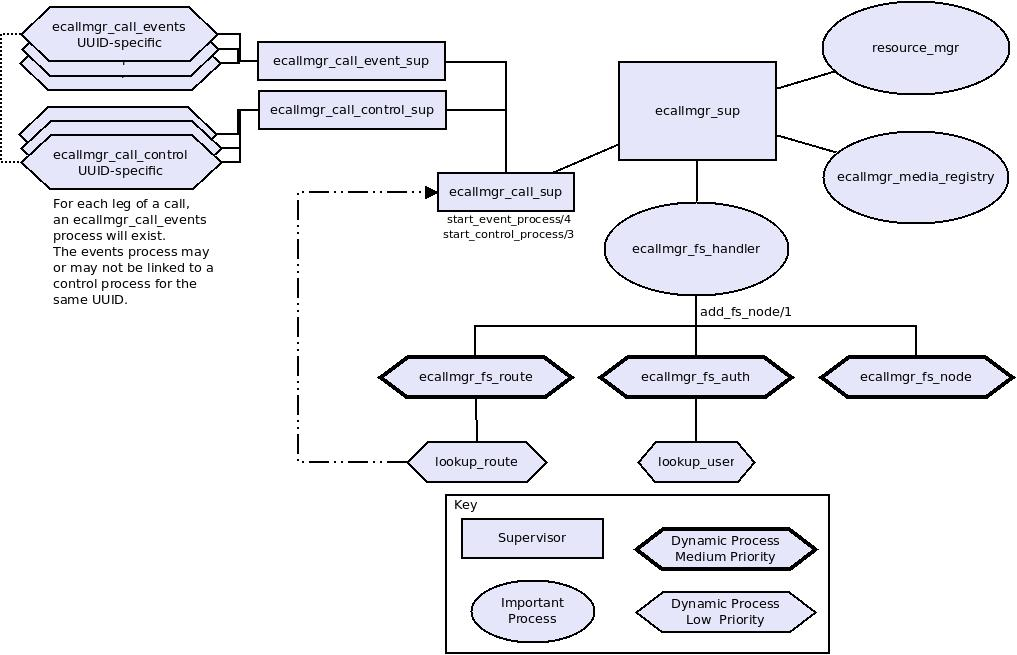
\includegraphics[width=\linewidth]{ecallmgr}
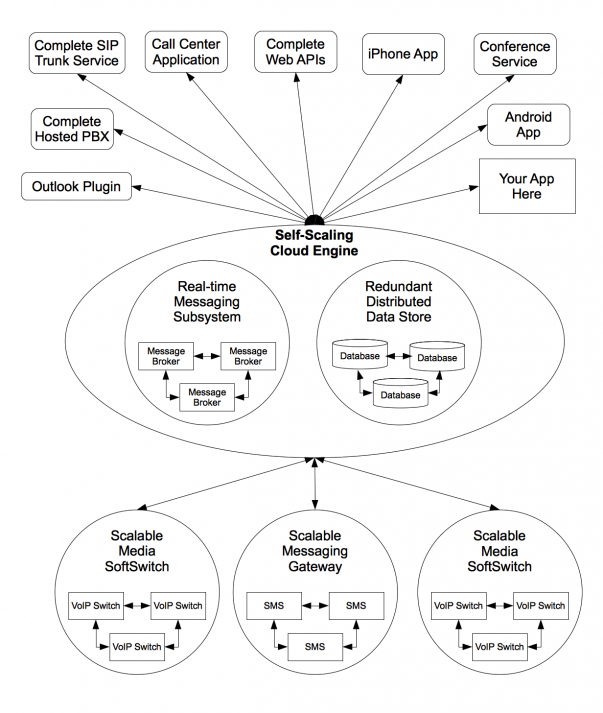
\includegraphics[width=\linewidth]{concept}